\documentclass{beamer}
\usepackage[spanish]{babel}
\usepackage[utf8]{inputenc}
\usepackage{graphicx}
\usepackage{color}
\newtheorem{definicion}{Definición}
\newtheorem{ejemplo}{Ejemplo}

%%%%%%%%%%%%%%%%%%%%%%%%%%%%%%%%%%%%%%%%%%%%%%%%%%%%%%%%%%%%%%%%%%%%%%%%%%%%%%%
\title[Método de Simpson]{\fbox{\fbox{Método de Simpson}}}
\author[Melanie, Nadia, Tania]{Melanie Hernández, Nadia Chinea, Tania Gutiérrez}
\date[17-05-2013]{17 de mayo de 2013}
%%%%%%%%%%%%%%%%%%%%%%%%%%%%%%%%%%%%%%%%%%%%%%%%%%%%%%%%%%%%%%%%%%%%%%%%%%%%%%%

%\usetheme{Madrid}
%\usetheme{Antibes}
%\usetheme{boxes}
%\usetheme{tree}
%\usetheme{classic}
\usetheme{Malmoe}

\usecolortheme{crane}
\useinnertheme{rounded}
\useoutertheme{shadow}
\usefonttheme{serif}

%%%%%%%%%%%%%%%%%%%%%%%%%%%%%%%%%%%%%%%%%%%%%%%%%%%%%%%%%%%%%%%%%%%%%%%%%%%%%%%
\begin{document}
  
%++++++++++++++++++++++++++++++++++++++++++++++++++++++++++++++++++++++++++++++  
\begin{frame}

%\includegraphics[=0.15\textwidth]{fmatesc.eps}
 \hspace*{7.5cm}
 
\includegraphics[width=0.16\textwidth]{logotipo-secundario-ULL.eps}
  \titlepage

  \begin{scriptsize}
    \begin{center}
     Facultad de Matemáticas \\
     Universidad de La Laguna
    \end{center}
  \end{scriptsize}

\end{frame}
%++++++++++++++++++++++++++++++++++++++++++++++++++++++++++++++++++++++++++++++  

%++++++++++++++++++++++++++++++++++++++++++++++++++++++++++++++++++++++++++++++  
\begin{frame}
  \frametitle{Índice}  
  \tableofcontents[pausesections]
\end{frame}
%++++++++++++++++++++++++++++++++++++++++++++++++++++++++++++++++++++++++++++++  




\section{Motivación y Objetivos}


%++++++++++++++++++++++++++++++++++++++++++++++++++++++++++++++++++++++++++++++  
\begin{frame}

\frametitle{Objetivo principal}
 
\begin{block}{}
La intención principal es el planteamiento de un experimento cuyo fin 
es el cálculo del área de una función dada de la forma más precisa posible. 
Interviene un método de integración numérica, por lo tanto conlleva no sólo un aprendizaje en el ámbito informático 
sino que además permite hacer un enfoque matemático 
que obliga a alcanzar una mayor destreza en este campo.

\end{block}
\end{frame}
%++++++++++++++++++++++++++++++++++++++++++++++++++++++++++++++++++++++++++++++  

%++++++++++++++++++++++++++++++++++++++++++++++++++++++++++++++++++++++++++++++  
\begin{frame}

\frametitle{Objetivos }

\end{frame}
%++++++++++++++++++++++++++++++++++++++++++++++++++++++++++++++++++++++++++++++  

\section{Fundamentos Teóricos}

\begin{frame}
\frametitle{Fundamentos Teóricos}

\end{frame}


\begin{frame}
\begin{block}{Fórmulas}
La fórmula simple se define como:
\[\int_{a}^{b} f(x)\text{d}x ~ \frac{b-a}{6}\big[f(a)+4f(m)+f(b)\big]\]\par
 
Por otra parte, la fórmula compuesta aparece como:

\[\int_{a}^{b} f(x)\text{d}x ~ \frac{h}{3}\big[f(x_0)+2\sum_{j=1}{\frac{n}{2-1}} f(x_{2j})+4 \sum_{j=1}{\frac{n}{2}}f(x_{2j-1})+f(x_n)\]

\end{block}

\end{frame}
%++++++++++++++++++++++++++++++++++++++++++++++++++++++++++++++++++++++++++++++  

\section{Procedimiento experimental}

\begin{frame}
\frametitle{Procedimiento experimental}
\begin{block}{}
El experimento se basará en la comparación entre las fórmulas, en el que se realizarán pruebas de tiempo de ejecución de ambas con 
diferentes intervalos,además de distintas reiteraciones en el caso de la compuesta.
Por lo tanto se puede dividir en dos partes.

\end{block}
\end{frame}
%++++++++++++++++++++++++++++++++++++++++++++++++++++++++++++++++++++++++++++++  

\subsection{Descripción de los experimentos}

%++++++++++++++++++++++++++++++++++++++++++++++++++++++++++++++++++++++++++++++  
\begin{frame}


\begin{ejemplo}
  \begin{itemize}
    \item Con 
    \item Con 
    \item Con 
  \end{itemize}
\end{ejemplo}

\end{frame}

\begin{frame}
\begin{block}{}

\end{block}
\end{frame}

%++++++++++++++++++++++++++++++++++++++++++++++++++++++++++++++++++++++++++++++  

\subsection{Descripción del material}
%++++++++++++++++++++++++++++++++++++++++++++++++++++++++++++++++++++++++++++++  
\begin{frame}
\frametitle{Hardware y Software}

\begin{ejemplo}
  \begin{enumerate}

      
  \end{enumerate}
\end{ejemplo}

\end{frame}
%++++++++++++++++++++++++++++++++++++++++++++++++++++++++++++++++++++++++++++++  

\subsection{Resultados obtenidos}
%++++++++++++++++++++++++++++++++++++++++++++++++++++++++++++++++++++++++++++++  
\begin{frame}
\frametitle{Medidas de tiempo y Velocidad}

%------------------------------------------------------------------------------
%--------------------------------------------------------------------------
\begin{table}[!ht]
\begin{center}
\begin{tabular}{|c||c||c|} \hline 
  \textbf{Intervalo} & \textbf{Area}  \\ \hline \hline
[-1,1] &  0693236856881
\\
\hline
[-1,4] & 0.633179114507
\\
\hline

[2,8] & 0.0539969133913
\\
\hline
\hline

\end{tabular}
\end{center}
\caption{Resultados experimentales del calculo del area (formula simple)}
\label{tab:1}
\end{table}


 %--------------------------------------------------------------------------
\begin{table}[!ht]
\begin{center}
\begin{tabular}{|c||c||c|} \hline 
\textbf{Intervalo} & \textbf{Area con iteracion = 4}  \\ \hline \hline
[-1,1] &  0.5813286
\\
\hline
[-1,4] & 0.646540956
\\
\hline

[2,8] & 0.0278711396576
\\
\hline
\hline

\end{tabular}
\end{center}
\caption{Resultados experimentales del calculo del area (formula compuesta)}
\label{tab:2}
\end{table}

%------------------------------------------------------------------------------

\end{frame}
%++++++++++++++++++++++++++++++++++++++++++++++++++++++++++++++++++++++++++++++  
%\begin{frame}

%\end{frame}

%++++++++++++++++++++++++++++++++++++++++++++++++++++++++++++++++++++++++++++++  
\begin{frame}
\frametitle{Representaciones de las funciones}

%------------------------------------------------------------------------------

\begin{figure}[!th]
\begin{center}
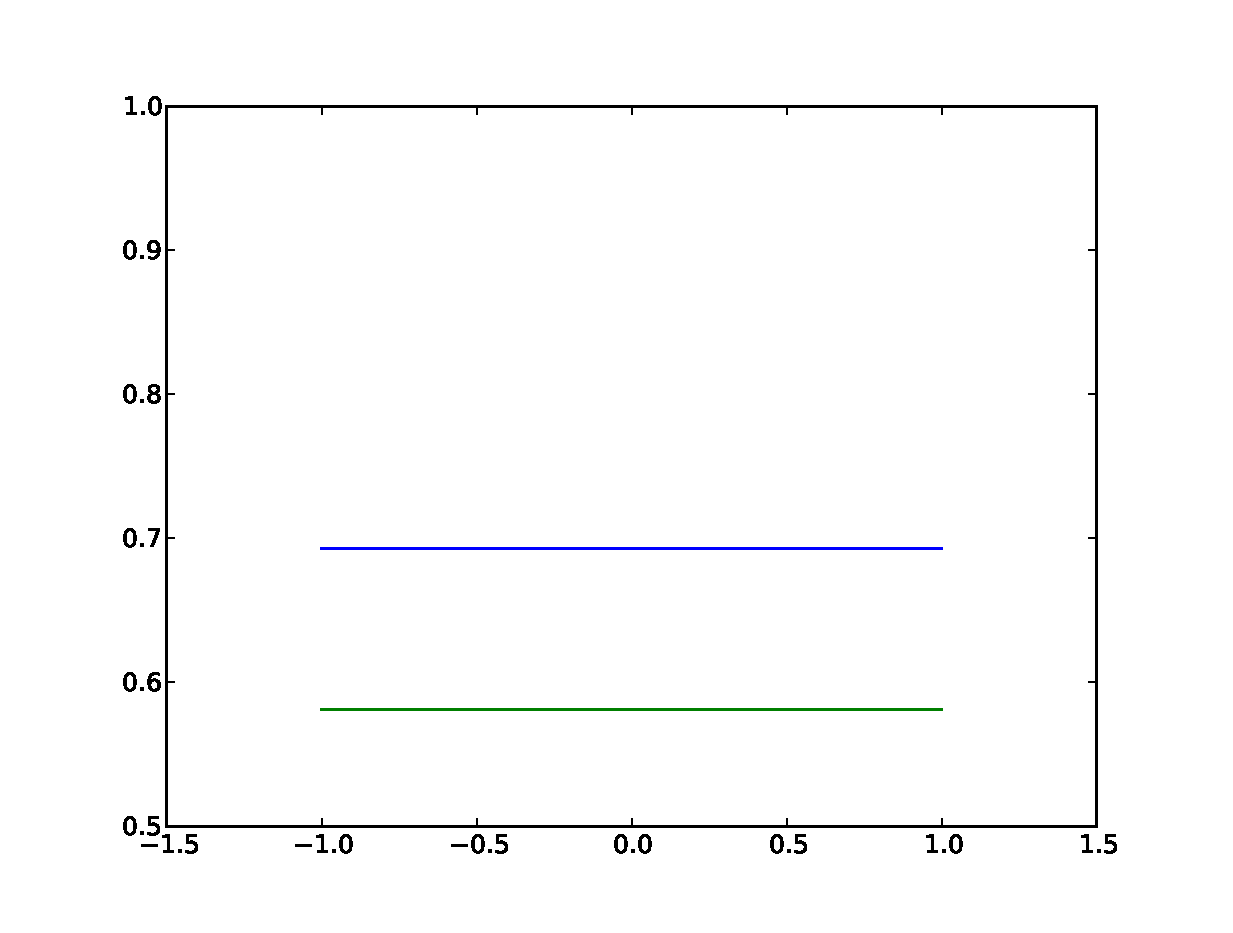
\includegraphics[width=0.75\textwidth]{1intervalo.eps}
\caption{Intervalo [-1,1]}
\label{fig:1}
\end{center}
\end{figure}


%------------------------------------------------------------------------------


%++++++++++++++++++++++++++++++++++++++++++++++++++++++++++++++++++++++++++++++  

\subsection{Análisis de los resultados}
\begin{frame}
\begin{block}{}
De las gráficas podemos decir que con los intervalos [-1,1] y [2,8], las rectas que 
se forman están más alejadas entre sí que en el intervalo que podríamos considerar ni grande ni pequeño. 
Se ha experimentado con el tiempo transcurrido para el tratamiento del método y con el de ejecución de la CPU. Como sabemos, el tiempo 
transcurrido durante la ejecución del programa varía dependiendo de la computadora que se use, aún así podemos apreciar que es mayor al realizar la fórmula 
compuesta debido a que las reiteraciones hacen que el programa se retase.
En cuanto al tiempo de la CPU, no varía en absoluto en ninguno de los intervalos porque la respuesta de la CPU es inmediata.
\end{block}


\end{frame}
\section{Conclusiones}

%++++++++++++++++++++++++++++++++++++++++++++++++++++++++++++++++++++++++++++++  
\begin{frame}
\frametitle{Conclusiones}

\end{frame}
%++++++++++++++++++++++++++++++++++++++++++++++++++++++++++++++++++++++++++++++  
%+++++++++++++++++++++++++++++++++++++++++++++++++++++++++++++++++++++++++++  

\end{document}